\nsecbegin{GUI-Anforderungen (Autor: Michael Lux)}
Denkanstöße:
\begin{itemize}
\item Wie könnte das User Interface aussehen?

\item Wie können wir für eine gute User Experience sorgen?
\end{itemize}
Auch, wenn die GUI im ersten Sprint nur in Grundzügen entwickelt wird, sollten wir uns früh Gedanken über deren Aussehen und Funktionalität machen. Dazu gehört, wie der Workflow abläuft und wie wir das GUI unserer Anwendung darauf zuschneiden können. Welche großen roten Knöpfe brauchen wir, welche Funktionen dürfen in dreifach verschachtelten Untermenüs versteckt werden?

Eine Möglichkeit fur das Aussehen und Funktionalität wäre folgende:

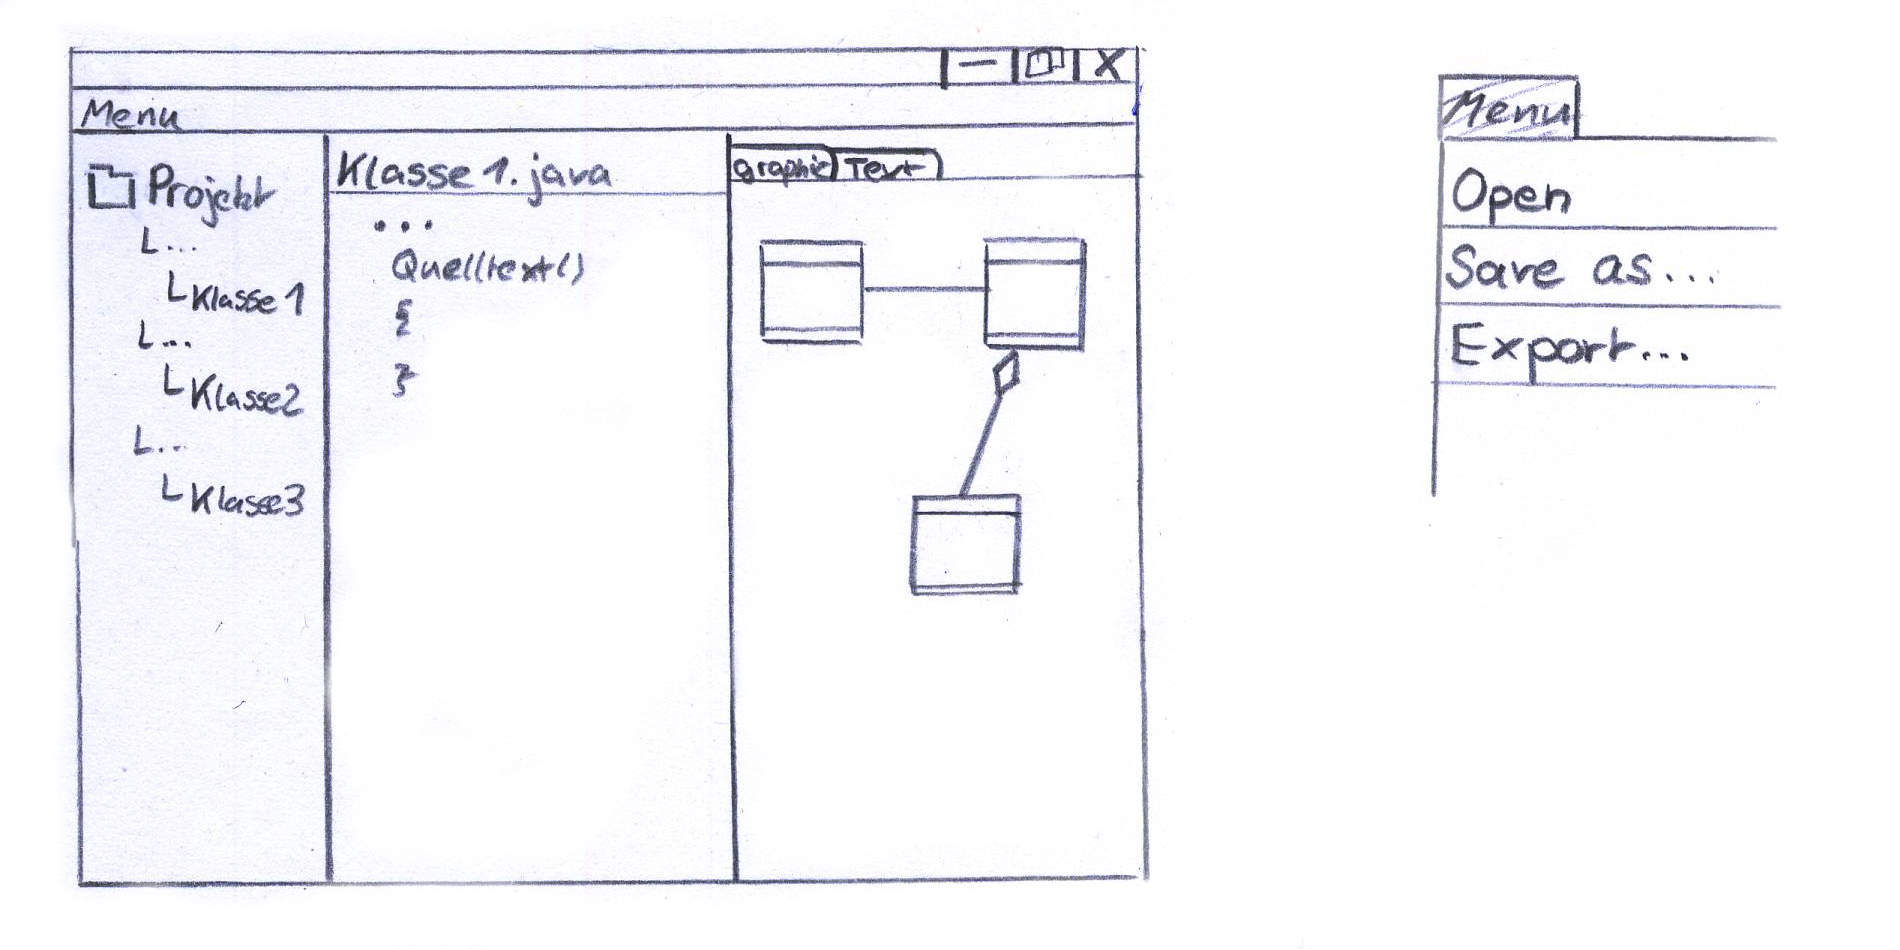
\includegraphics[]{Bilder/GUI-Beispiel.png}

Die wichtigsten Funktionalitäten verbergen sich im Untermenü unter Menü.
Ein Projekt bzw. eine Datei mit verschiedenen Klassen soll dort unter „Open“ geöffnet werden.
Das Programm erzeugt daraus automatisch die UML, die rechts entweder grafisch, oder in Textform dargestellt wird. (Auswahl durch Tabs)
Links ist die Klassenhierarchie und der Quelltext der jeweiligen Klasse bzw. Datei zu sehen.
Die erstellte UML soll durch den Benutzer per Maus- und Tastatureingaben in der UML selbst verändert werden können. (Beispiel: Verschieben einer Klasse mit der Maus)
Anschließend soll der Anwender die Möglichkeit haben, die UML grafisch als Bilddatei oder in Textform speichern zu können über die Funktionen „Save as“ und „Export“.
\nsecend